\documentclass{beamer}
%
% Choose how your presentation looks.
%
% For more themes, color themes and font themes, see:
% http://deic.uab.es/~iblanes/beamer_gallery/index_by_theme.html
%
\mode<presentation>
{
  \usetheme{default}      % or try Darmstadt, Madrid, Warsaw, ...
  \usecolortheme{whale} % or try albatross, beaver, crane, ...
  \usefonttheme{default}  % or try serif, structurebold, ...
  \setbeamertemplate{navigation symbols}{}
  \setbeamertemplate{caption}[numbered]
} 

\usepackage{listings}
\usepackage[english]{babel}
\usepackage[utf8x]{inputenc}
\usepackage{makecell}

\title{Quantum A-Star Search}
\subtitle{Presenting a Novel Grover's Based Approach to Optimal Path Findi}
\author{Sam Bieler, Michael Tylko, Eli Shieber}
\institute{ES 170 | Professor Pri}
\date{May 8, 2019}

\begin{document}

\begin{frame}
  \titlepage
\end{frame}

% Uncomment these lines for an automatically generated outline.
%\begin{frame}{Outline}
%  \tableofcontents
%\end{frame}

\begin{frame}{Optimal Pathfinding}

\begin{block}{Problem Statement}
\begin{itemize}
  \item Given a set of nodes, $N$, a set of edges, $E$, a start node, $S$, and a goal node, $F$, what is the optimal route to traverse from start to goal?
  \item Let $f: E \rightarrow \mathbb{R}$ represent a function from edge to edge cost.
  \item Let $e_{ij}$ be the edge between node $i$ and node $j$.
  \item Our goal is then to find a path, $P = (e_{Si},...,e_{jF})$, for which we minimize the objective:
  $$ \sum_{e_{ij} \in P} f(e_{ij}) $$
\end{itemize}
\end{block}
\end{frame}

\begin{frame}{Grid World Problem Set Up}

\begin{block}{Grid World}
\begin{itemize}
  \item We frame the graph for this path finding problem by establishing a grid 
\end{itemize}
\end{block}
\end{frame}

\begin{frame}{Classical A-Star Search}

\begin{block}{Individual Possessions as a Markov Chain}
\begin{itemize}
  \item Each possession is comprised of a set of discrete events such as passes, fouls, shot attempts, and turnovers.
  \item We make the assumption that our  system adheres to the Markov property as the state transition probabilities only depend on the system’s current state.
  \item 36-state Markov chain: 1 Team state, 5 player possession states, 25 player action states (5 for each), 3 scoring states, 1 offensive rebound, and 1 final end of possession.
\end{itemize}
\end{block}
\end{frame}





\begin{frame}{Controlled Z-Gate Implementation}

\begin{block}{4 Qubit Case}
%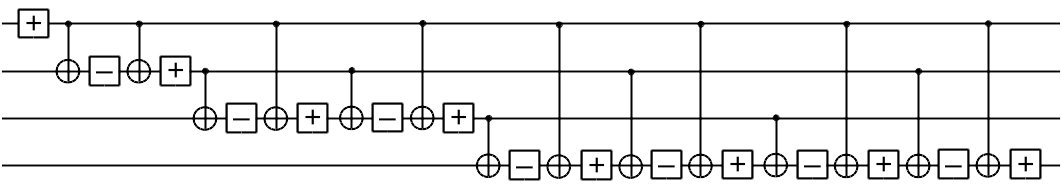
\includegraphics[width=11cm]{4qubitcontrolledzgate.jpg}
\end{block}

\begin{block}{The Pattern}
\begin{itemize}
  \item 0
  \item 0,1,0
  \item 0,1,0,2,0,1,0
  \item 0,1,0,2,0,1,0,3,0,1,0,2,0,1,0
\end{itemize}
\end{block}

\end{frame}


\begin{frame}{Controlled Z-Gate Implementation Continued}
\begin{block}{The Code}
\end{block}
\end{frame}

\begin{frame}{Model Description}
\begin{block}{Transition Probabilities}
\begin{itemize}
    \item We assume that the ball will be randomly and evenly distributed amongst the five players on a change of possession.
    \item We also assume that any given player will pass the ball to another teammate 80\% of the time,  while taking an action in the remaining 20\% of the time.
\end{itemize}
\end{block}
\begin{block}{Cross Player Passing Probabilities}
\begin{itemize}
    \item Conditional on a player deciding to pass the ball we determine who the pass goes to by developing player usage statistics.
    \item We compare minutes played per game (MPG) and average points per possession to calculate an offensive importance measure (OIM) from which we will calculate each player’s usage.
\end{itemize}
\end{block}
\end{frame}

\begin{frame}{Model Description}
\begin{block}{Cross Player Passing Probabilities}
\begin{itemize}
    \item For example, the usage rates for Golden State’s $n= 5$ starters in 2018 are computed as follows:
\end{itemize}

$$ OIM = MPG \cdot (2\cdot2\mbox{P}+3\cdot3\mbox{P}),\ \ \text{Usage}_i = \frac{OIM_i}{\sum_{n} OIM_n}  $$

\vspace{-3mm}

\begin{table}[H]
\centering
\begin{tabular}{|l|l|l|l|l|l|} 
\hline
Player          & MPG & 2P   & 3P  & OIM     & Usage  \\ 
\hline
Kevin Durant    & 34.2                    &  9.5 & 3.6 & 1018.90 & 0.27   \\ 
\hline
Steph Curry      & 32                      & 6.4  & 6.3 & 1013.78  & 0.27   \\ 
\hline
Klay Thompson   & 34.3                    &  6.7  & 4.4 & 913.15  & 0.24   \\ 
\hline
Draymond Green & 32.7                   & 4.3  & 1.6 & 437.80  & 0.12   \\ 
\hline
Quinn Cook     & 22.4                    & 4.9  & 3.0 & 421.58  & 0.11   \\
\hline
\end{tabular}
\end{table}
\end{block}
\end{frame}


\begin{frame}{Model Description}
\begin{block}{Non-Pass Action Probabilities}
\begin{itemize}
    \item Conditional on the player deciding not to pass, we split up the transition probabilities based on these statistics.
    \item For example, per 100 possessions LeBron James will take 6.6 3-point attempts, 19.0 2-point attempts, 8.6 free throw attempts, and have 5.6 turnovers.
    \item We then use this distribution to set proportions for the actions accordingly. We assume exactly 2 free throws are awarded for each foul, such that the total number of actions for LeBron James is $6.6+19.0+8.7/2+5.6=35.55$.
    \item The corresponding probability of, for instance, a 2-point attempt is $19.0/35.55=0.5344$ given that he is the player that decides to take the action.
\end{itemize}
\end{block}
\end{frame}

\begin{frame}{Model Description}
\begin{figure}
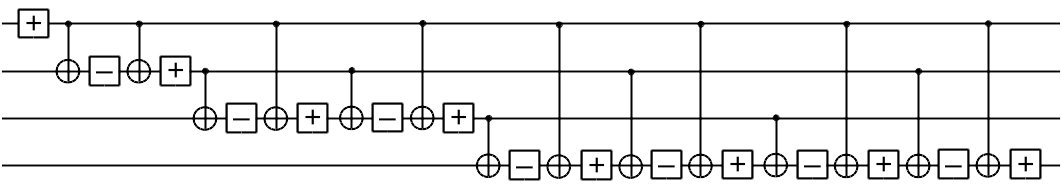
\includegraphics[width=10cm]{4qubitcontrolledzgate.jpg}
\end{figure}
\end{frame}

\begin{frame}{Model Extension 1}
\begin{block}{Adjusting for Opponent's Defensive Ability}
\begin{itemize}
    \item To improve our model's fidelity we adjust our shot success rates to encode the strength of the defense.
    \item Using NBA team summary statistics, we compare a team's 2- and 3-point percentages against to the league average.
    \item We then use these comparisons to adjust the offensive success rates when matched against a given team.
    \item A player's 2-point shooting \% is adjusted by a factor of the opposing team's 2-point field goal \% against divided by the league average 2-point field goal \% against
\end{itemize}

$$2\mbox{P}\%_{\mbox{Player}}=\frac{2\mbox{P_{\mbox{Player}}}}{2\mbox{PA}_{\mbox{Player}}}\cdot\bigg(\frac{2\mbox{P}\%_{\mbox{Opp}}}{2\mbox{P}\%_{\mbox{League}}}\bigg)$$

\end{block}
\end{frame}

\begin{frame}{Model Extension 2}
\begin{block}{Encoding Bench Substitutions}
\begin{itemize}
    \item It is unrealistic for the entire game to be played by the same 5 players from each team, so we also allow for the bench to be substituted in at different points of the game.
    \item We chose to put all 10 substitutes (5 from each team) in the game during two different portions of the game: between possessions 49 and 72 and possessions 121 and 144.
\end{itemize}
\end{block}
\end{frame}

\begin{frame}{Model Extension 2}
\begin{block}{Encoding Bench Substitutions}
\begin{itemize}
    \item Figure 1 and Figure 2 show how game score progression.
    \item Areas in between the dotted lines show the possessions for which each team put in their designated substitutes.
\end{itemize}
\end{block}
\begin{figure}[!htb]
   \begin{minipage}{0.5\textwidth}
     \centering
     \includegraphics[width=\linewidth]{examplesim2.png}
     \caption{Cleveland vs. Boston in 2018}
   \end{minipage}\hfill
   \begin{minipage}{0.5\textwidth}
     \centering
     \includegraphics[width=\linewidth]{examplesim.png}
     \caption{Houston vs. Golden State in 2019}
   \end{minipage}
\end{figure}
\end{frame}



\begin{frame}{Sensitivity Analysis}

\begin{itemize}
    \item We measured our model's sensitivity against changes in which player starts with the ball and the passing rate between the players on the court
    \item We found little change in offensive output from varying these parameters
    
\end{itemize}

\begin{figure}[!htb]
   \begin{minipage}{0.5\textwidth}
     \centering
     \includegraphics[width=\linewidth]{sens_start.png}
   \end{minipage}\hfill
   \begin{minipage}{0.5\textwidth}
     \centering
     \includegraphics[width=\linewidth]{sens_pass.png}
   \end{minipage}
\end{figure}
\end{frame}

\begin{frame}{Sensitivity Analysis}

\begin{itemize}
    \item Our model was quite sensitive to defensive rebounding rate, which we treated as a constant across all teams
    \item We chose a rate of 0.75 to reflect league averages and typical points per game values
    
\end{itemize}

\begin{figure}
\includegraphics[width=6.7cm]{sens_def.png}
\end{figure}
\end{frame}

\begin{frame}{Fundamental Matrix Analysis}
\begin{itemize}
    \item As shown in lecture, we can reveal some interesting features of our system by placing our transition matrix in canonical form and computing the fundamental matrix, $N = (I-Q)^{-1}$.
\end{itemize}
\begin{figure}
    \centering
    \includegraphics[width=6cm]{canon.png}
\end{figure}
\end{frame}

\begin{frame}{Fundamental Matrix Analysis}
\begin{itemize}
    \item By looking at the sum of the columns of $N$ we can find the expected number of transitions before absorption for each non-absorbing start state. 
    \item Below we can see the expected number of steps before absorption conditional on starting the possession with a given player for GSW (vs CLE) in 2018:
\end{itemize}

\vspace{-2mm}

\begin{table}[H]
\centering
\begin{tabular}{l|l|l|l|l|l}
         & KD & SC & KT & DG & QC \\ \hline
Steps to Absorption  & 6.8294   & 6.8362   & 6.8488   & 6.8105   & 6.8453   \\
\end{tabular}
\caption{Expected Steps to Absorption Conditional on Starting Player}
\end{table}
\end{frame}

\begin{frame}{Fundamental Matrix Analysis}
\begin{itemize}
    \item We can also compute the probability of absorption in a certain absorbing state given that the process starts at a certain player by examining $B=R\cdot N$.
    \item Starting with Curry or Thompson slightly increased the odds of making a 3-point shot.
    \item Starting with Green start with possession led to a slightly higher chance of not scoring on the possession.
\end{itemize}
\begin{table}[H]
\centering
\begin{tabular}{l|l|l|l|l|l}
         & KD & SC & KT & DG & QC \\ \hline
P(1 pt)  & .0113   & .0107   & .0099   & .0127   & .0098   \\ \hline
P(2 pts) & .3771   & .3587   & .3587   & .3591   & .3598   \\ \hline
P(3 pts) & .1583   & .1742   & .1717   & .1542   & .1691   \\ \hline
P(0 pts) & .4533   & .4565   & .4596   & .4740   & .4613   \\ 
\end{tabular}
\caption{Expected Absorption Outcome Conditional on Starting Player}
\end{table}
\end{frame}

\begin{frame}{Fundamental Matrix Analysis}
\begin{itemize}
    \item This chart demonstrates the tendency for the ball to be passed around for roughly 6 steps, confirming what we saw above.
    \item We also see roughly the same breakdown of final absorbing states given as we saw with our fundamental matrix analysis.
\end{itemize}
\begin{figure}
    \centering
    \includegraphics[width=10cm]{state_dist.png}
\end{figure}
\end{frame}


\begin{frame}{2018 Playoff Simulation}

\begin{itemize}
    \item We looked at 51 game simulations between the two teams to better control for randomness
    \item Our model predicted all but one first round match up correctly (Cleveland ultimately made it to the final)
    \item This also correctly predicted two Western Conference upsets: New Orleans over Portland and Utah over Oklahoma City
\end{itemize}

\vspace{-3mm}

\begin{figure}
\includegraphics[width=11cm]{2018_sim.png}
\caption{2018 NBA Playoffs | Simulated Results}
\end{figure}
\end{frame}

\begin{frame}{2019 Playoff Simulation}

\begin{itemize}
    \item Again looking at 51 game simulations, our model predicts that Golden State will win the championship for the third consecutive year
    \item Our model predicts two big upsets: Oklahoma City over Denver and Boston over Milwaukee
\end{itemize}

\vspace{-5mm}

\begin{figure}
\includegraphics[width=11cm]{2019_sim.png}
\caption{2019 NBA Playoffs | Simulated Results}
\end{figure}
\end{frame}


\begin{frame}{Predictions for NBA Champion}
\begin{itemize}
    \item We ran 50 simulations of the 2018 and 2019 playoffs
    \item Golden State came out on top over a third of the time - equivalent to 2:1 odds
\end{itemize}

\begin{figure}[!htb]
   \begin{minipage}{0.5\textwidth}
     \centering
     \includegraphics[width=\linewidth]{2018.png}
   \end{minipage}\hfill
   \begin{minipage}{0.5\textwidth}
     \centering
     \includegraphics[width=\linewidth]{2019.png}
   \end{minipage}
\end{figure}
\end{frame}


\begin{frame}{Future Work}
\begin{itemize}
    \item \textbf{Playoff Effects:} A team's best players often handle the ball significantly more in the playoffs when each game's importance is amplified. Our usage statistics only capture regular season tendencies and may not be accurate for simulating the playoffs. 
    \item \textbf{Finite Shot Clock:} Our model fails to consider the time of each step in the Markov chain. With a 24-second shot clock, certain possessions might time out if a decision is not made quickly enough, or decisions may even be influenced by the time.
    \item \textbf{In-Game Strategy Changes:} Teams may substitute out a player who is having a poor game or shift their gameplan towards taking more of a certain type of shot if it has been successful during the game.

\end{itemize}
\end{frame}

\end{document}
